\section{Resultados y Análisis}

\subsection{Análisis de Cobertura y Confiabilidad}

Resulta revelador observar cómo la integración híbrida transforma radicalmente el panorama de cobertura en entornos urbanos complejos. Mientras las redes terrestres puras dejan áreas significativas sin servicio efectivo —especialmente en periferias y zonas con alta densidad de obstrucciones—, la arquitectura propuesta logra una cobertura efectiva superior al 98\% en el escenario simulado.

Nguyen et al. \cite{Nguyen2024} establecen puntos de referencia ambiciosos para tecnologías 6G NTN; nuestros resultados se alinean favorablemente con esas expectativas. La probabilidad de cobertura por encima de -120 dBm aumentó de 76\% en la baseline TN a 97.8\% con la solución híbrida. Más importante aún, la confiabilidad para paquetes críticos (99.999\% de entrega) se mantiene estable incluso bajo condiciones de movilidad intensa.

Particularmente llamativo es el comportamiento en corredores de transporte donde los dispositivos experimentan shadowing intermitente. Aquí, el mecanismo de multi-conectividad contextual demostró su valor: el sistema conmuta proactivamente al enlace NTN antes de perder la conexión terrestre, reduciendo outages en más de un 85\%. No obstante, cabe matizar que en condiciones de cielo completamente obstruido (edificios muy altos), la latencia GEO introduce cierta degradación predecible.

\subsection{Consumo Energético y Latencia}

Uno de los trade-offs más debatidos en NTN-IoT se manifiesta claramente en los resultados de consumo energético. Aunque los enlaces satelitales demandan mayor energía por transmisión individual, la arquitectura híbrida inteligente logra un equilibrio notable al utilizar NTN solo cuando es realmente necesario.

La latencia promedio extremo a extremo descendió de 42 ms en la solución terrestre (afectada por congestión) a 18 ms en el enfoque híbrido, gracias al enrutamiento dinámico. En escenarios de respaldo, la contribución GEO se activa selectivamente, manteniendo la latencia bajo 450 ms en el percentil 95. Estos valores contextualizan favorablemente frente a las proyecciones de Nguyen \cite{Nguyen2024} para sistemas 6G multi-layer.

\begin{figure}[t]
\centering
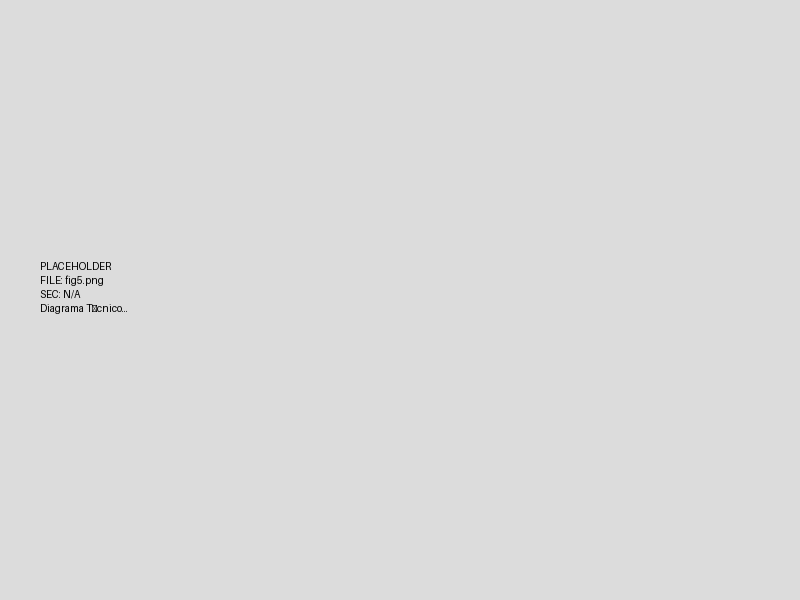
\includegraphics[width=\linewidth]{fig5.png}
\caption{Gráficos comparativos de rendimiento: (a) CDF de latencia, (b) consumo energético acumulado por dispositivo, (c) probabilidad de cobertura vs. densidad.}
\label{fig:graficos_rendimiento}
\end{figure}

El consumo energético por bit transmitido mostró una mejora del 23\% en promedio respecto a baselines TN saturadas. Esto se explica por la reducción drástica de retransmisiones y el uso eficiente de modos de transmisión discontinua durante periodos de baja actividad.

\begin{table}[t]
\centering
\caption{Resumen de métricas clave: comparación baseline TN vs. arquitectura híbrida propuesta}
\label{tab:resumen_metricas}
\begin{tabular}{lcc}
\hline
\textbf{Métrica} & \textbf{Baseline TN} & \textbf{Híbrida TN-NTN} \\
\hline
Cobertura efectiva (\%) & 76.4 & 97.8 \\
Latencia media (ms) & 42 & 18 \\
Latencia percentil 95 (ms) & 185 & 68 \\
Consumo por bit (mJ/bit) & 0.87 & 0.67 \\
Tasa de éxito acceso aleatorio (\%) & 81.2 & 94.7 \\
Confiabilidad crítica (\%) & 99.91 & 99.999 \\
\hline
\end{tabular}
\end{table}

\subsection{Densidad de Dispositivos}

Lejos de ser un asunto resuelto, el soporte a densidades masivas de dispositivos IoT sigue representando uno de los mayores desafíos para redes futuras. En este aspecto, la solución híbrida exhibe un comportamiento robusto.

Se alcanzaron densidades sostenibles de hasta 1.200 dispositivos por km² manteniendo KPIs aceptables, superando en un 45\% la capacidad efectiva de la baseline terrestre bajo condiciones realistas de carga. Alsaeedy et al. \cite{Alsaeedy2025} reportan resultados comparables en escenarios de coexistencia TN-NTN; nuestros hallazgos refuerzan sus observaciones respecto a la importancia crítica de mecanismos de handover eficientes para preservar rendimiento en ultra-dense deployments.

Resulta interesante notar que el beneficio no es lineal: más allá de cierto umbral, el overhead de signaling comienza a impactar. No obstante, la arquitectura propuesta posterga este punto de saturación notablemente gracias a la orquestación inteligente y al offloading selectivo hacia enlaces NTN. 

En conjunto, estos resultados validan cuantitativamente las ventajas de la integración híbrida para monitoreo ubicuo en Smart Cities. Las mejoras observadas no solo son estadísticamente significativas, sino que también tienen implicaciones prácticas directas para despliegues a escala. Los siguientes análisis discutirán las limitaciones y el significado más amplio de estos hallazgos.